\documentclass[12pt,a4paper] {article}

\pagestyle{empty}

\usepackage[TD]{../../../Style}

%\renewcommand{\baselinestretch}{1.25}


\begin{document}

\titre{Comparaison d'épidémies}

Dans un monde imaginaire, deux virus pour l'instant bénins ont fait leur apparition.
\begin{itemize}
\item Le premier, intitulé le \textit{"Bovide"}, a déja touché vingt millions de personnes dans le monde et en touche vingt millions de plus chaque jour.
\item Le second,  baptisé \textit{"Grippe abière"} n'a pour l'instant touché qu'une famille de 5 individus mais les études montrent que la quantité de personnes infectées est multipliée par $1.2$ chaque jour (on ne tiendra pas compte des décimales qui apparaitront).
\end{itemize}
Cependant, le budget alloué à la recherche d'un vaccin n'est pas suffisant pour étudier les deux virus et un choix doit être fait. C'est pour cela que le gouvernement fait appel à la \premiere ST2S 2 du lycée Jean Rostand pour lui venir en aide.

On note respectivement $b_n$ et $g_n$ le nombre de personnes touchées au $n$-ème jour respectivement par le bovide et par la grippe abière (on part du jour 0). Ainsi, $b_0=20 \ 000 \ 000, \ b_1=40 \ 000 \ 000$, et $g_0=5, \ g_1=6$.

\begin{enumerate}
\item Compléter les schémas suivants:

\begin{center}
\begin{tikzpicture}[scale=1.7]
\node[draw,,ellipse,thick, minimum size=15mm] (W0) at (-3,0) {$b_0=20 \ 000 \ 000$};
\node[draw,,ellipse,thick, minimum size=15mm] (W1) at (0,0) {$b_1=40 \ 000 \ 000$};
\node[draw,,ellipse,thick, minimum size=15mm] (W2) at (3,0) {$b_2=\makebox[2cm]{\dotfill}$};
\node (W5) at (6,0) {$\ldots$};
\draw[->,>=latex,thick] (W0) to[bend left=20] node[midway,above]{$+ \makebox[1.8cm]{\dotfill}$} (W1);
\draw[->,>=latex,thick] (W1) to[bend left=20] node[midway,above]{$+ \makebox[1.8cm]{\dotfill}$} (W2);
\draw[->,>=latex,thick,densely dashed] (W2) to[bend left=20] node[midway,above]{$+ \makebox[1.8cm]{\dotfill}$} (W5);
\end{tikzpicture}
\end{center}

\begin{center}
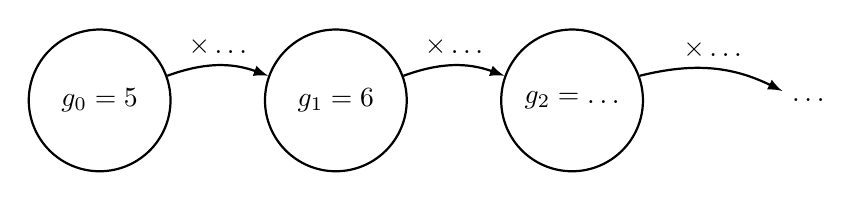
\begin{tikzpicture}[scale=1]
\node[draw,circle,thick, minimum size=18mm] (W0) at (-3,0) {$g_0=5$};
\node[draw,circle,thick, minimum size=18mm] (W1) at (0,0) {$g_1=6$};
\node[draw,circle,thick, minimum size=18mm] (W2) at (3,0) {$g_2=\ldots$};
\node (W5) at (6,0) {$\ldots$};
\draw[->,>=latex,thick] (W0) to[bend left=20] node[midway,above]{$\times \ldots$} (W1);
\draw[->,>=latex,thick] (W1) to[bend left=20] node[midway,above]{$\times \ldots$} (W2);
\draw[->,>=latex,thick] (W2) to[bend left=20] node[midway,above]{$\times \ldots$} (W5);
\end{tikzpicture}
\end{center}

\item Déterminer une relation de récurrence vérifiée par les suites $(b_n)$ et $(g_n)$:

\hfill {$b_{n+1}=b_n+\ldots$} \hfill {$g_{n+1}=g_n \times \ldots$} \hfill \

\item Ouvrir un tableur.
\item \begin{enumerate}
\item Dans la cellule A1, écrire \verb|Jour n|.
\item Rentrer 0 dans la cellule A2.
\item Cliquer sur la cellule A2. Un carré noir apparait alors en bas à droite de la cellule. Cliquer et glisser ce carré vers le bas pour le relâcher sur la cellule A120.
\end{enumerate}
\item \begin{enumerate}
\item Dans la cellule B1, écrire \verb|Bovide: b_n|.
\item Dans la cellule B2, écrire le premier terme de la suite $(b_n)$.
\item Ecrire dans la cellule B3 la relation de récurrence: \ \verb|=B2+20000000|.
\item Cliquer sur la cellule B3. Un carré noir apparait alors en bas à droite de la cellule. Cliquer et glisser ce carré vers le bas pour le relâcher sur la cellule B120.
\item Lire sur le tableur la valeur de $b_{10}$, de $b_{50}$.
\end{enumerate}
\item Procéder de même avec la suite $(g_n)$ sur la colonne C. On utilisera la formule: \ \verb|=B2*1.2|. Pour avoir une meilleure lisibilité, on pourra sélectionner la colonne C, faire un clic droit puis "Formater des cellules", puis mettre le nombre de décimales à 0.
\item En combien de temps chaque virus contaminera un million de personnes? Cent millions? Un milliard? Quel virus est le plus dangereux à court terme? A long terme?
\item En combien de temps la grippe abière contaminera-t-elle l'humanité? (Environ 7.9 milliard d'individus)
\item Réaliser un graphe représentant ces deux suites: Selectionner les colonnes $B$ et $C$, puis dans le menu en haut de la fenêtre, cliquer sur "Données", puis "Diagramme" et enfin "Terminer".
\item A la suite d'une mutation au trentième jour, les deux virus deviennent extrêmement mortels. Ils ont maintenant un taux de mortalité journalier de $18 \%$ ( c'est-à-dire que $18 \%$ des contaminés meurent chaque jour ), quel virus serait alors le plus dangereux?
\end{enumerate}

%\rem[black]{Pour le covid c'était pas 1.2 mais entre 0.8 et 2.8 pour les pires moments !}


%Valeurs a modifier : 20 millions et 1.1 par ex

\end{document}
